\chapter{Some Mathematica scripts}
\label{app:mathematica}

In this appendix, we give as examples of the work that was done during the internship, some ``representative'' excerpts from our Mathematica scripts.

\section{Computation of the anomalous dimensions}

We showed in section \eqref{sec:etaperp} that 
\begin{align}
\eta_\perp = \frac{1}{Z_\perp} \tr{\Pi^r_{\cdot \cdot} \Gamma^{(3)}_{\cdot2\cdot} \Pi^a_{\cdot \cdot} \Gamma^{(3)}_{\cdot2\cdot}} \hat{\p{t}} \lim_{p \rightarrow 0} \frac{d}{dp^2_\perp} \int_q G_r(q) G_a(p+q)
\end{align}
We still need to let the derivative with respect to $p^2$ act on the massless propagator $G_a(p+q)$, and then to take the limit $p \rightarrow 0$. This is extremely cumbersome to do by hand, so we used Mathematica to do the expansion.

We start by defining our own scalar product, $scal$. It is defined to be symmetric in its two arguments, and linear. These are the only properties of a scalar product we are going to need.
\begin{lstlisting}
SetAttributes[scal, Orderless];
scal[a_ b_, c_] /; NumberQ[a] := a scal[b, c];
scal[a_ + b_, c_] := scal[a, c] + scal[b, c];
scal[0, a_] := 0;
\end{lstlisting}

The scalar products appears inside an integral over an internal momentum $q$. Since the integrand is invariant by rotation, the scalar products can be simplified. We designed replacement rules to take into account this simplifications:
\begin{lstlisting}
integr1 = {scal[ps, qs]^2 -> 1/m scal[ps, ps] scal[qs, qs],  
	scal[ps, qs]^4 -> 3/(m (m + 2)) (scal[ps, ps] scal[qs, qs])^2};
integr2 = {scal[ps, qs] -> 0};
\end{lstlisting}

Then we give to Mathematica the expression of the massless propagator
\begin{lstlisting}
G = (Zs scal[ps + qs, ps + qs]^2 + Zp scal[qp, qp] + rho0 scal[ps + qs, ps + qs] 
	+ R[scal[ps + qs, ps + qs], scal[qp, qp]] + U')^-1;
\end{lstlisting}

We are now ready to expand the propagators in powers of the scalar product, to take the derivative with respect to $p^2$ and take the limit of vanishing external momentum:
\begin{lstlisting}
Series[Series[G, {scal[ps, ps], 0, 2}] // Normal,
	 {scal[ps, qs], 0,  4}] // Normal;
% /. integr1;
% /. integr2;
(1/2)*D[%, {scal[ps, ps], 2}];
% /. ps -> 0;
\end{lstlisting}

After that, we obtain an expression that can still be simplified a little bit by integration by parts, to give the final form of eq. \eqref{eq:flow_perp}.

\section{Integration of the fixed point equations}

As a second example, we give the loop used to produce graphs of the ``explosion time'' of the potential as a function of the initial condition on the fixed point equation.
The integration is stopped when the $"Event"$ is triggered. Here it is when denominator of the massive propagator explodes; as this was found to be the condition met at the explosion time.
\begin{lstlisting}
Do[
 xsing = 0;
 NDSolve[{0 == equ[x, rho0, 1/2, 0], 
   u[0] == (n b1[1/2, 0] b2[1/2, 0, rho0])/(1 + sig), 
   u'[0] == sig}, u, {x, 0, xfin}, 
  Method -> {"EventLocator", 
    "Event" -> (-1 + n) /(1 + rho0 + u'[x]) + 
    (-u[x] + x a[1/2, 0] u'[x])/(b1[1/2, 0] b2[1/2, 0, rho0] ) , 
    "EventAction" :> {Throw[xsing = x, "StopIntegration"]}, 
    Method -> "BDF"}, AccuracyGoal -> 30];
 AppendTo[xs, {sig, xsing}];
 , {sig, sigList}]
 \end{lstlisting}

This produces the graph below, showing the neighborhood of the Lifshitz point in $d=3$.
\begin{figure}[htp]
\begin{center}
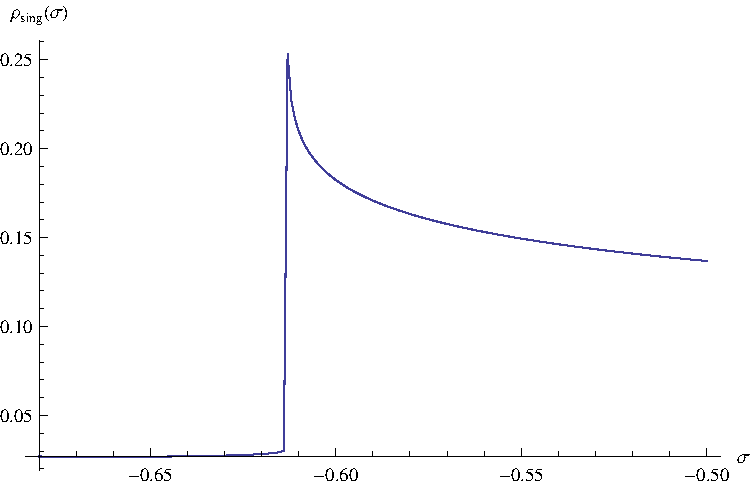
\includegraphics[scale=0.75]{img/app_mathematica/result.pdf}
\caption{The singularity location $\rho_{\text{sing}}$ as a function of the temperature $u'(\rho=0) = \sigma$, in the neighborhood of the Lifshitz point, with $d=3$, $m=1$.}
\label{}
\end{center}
\end{figure}